\section{Exercise 2: AM Simulation}
\label{sec:ex2}

\subsection*{Objective}
Integrate the AM modulator and both demodulation sub-VIs in a single top-level simulation and compare coherent versus envelope detection as the modulation index changes.

\subsection*{Top-Level Design}
The top-level AM simulation VI is shown in Figure~\ref{fig:am_top_level}.
\begin{figure}[H]
\centering
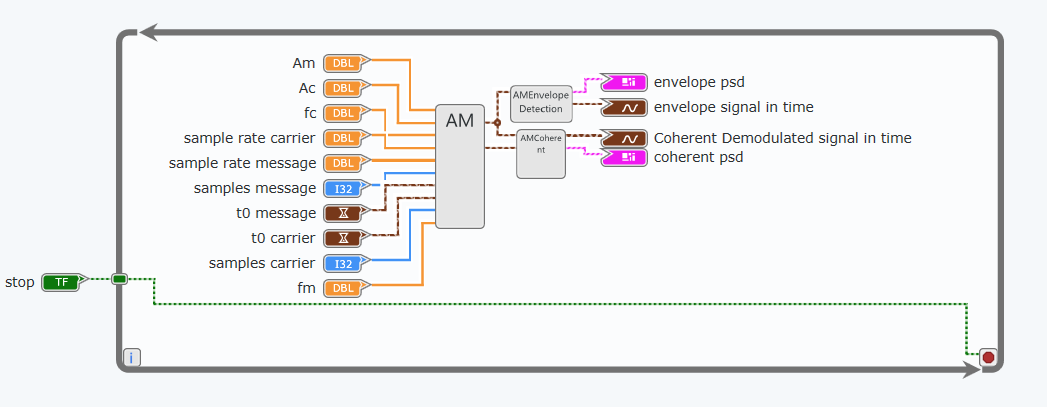
\includegraphics[width=\linewidth]{figures/AM_top_level.png}
\caption{Top-level AM simulation VI connecting modulation, coherent demodulation, and envelope detection.}
\label{fig:am_top_level}
\end{figure}

The top-level VI:
\begin{itemize}
\item generates an AM waveform from message and carrier parameters,
\item passes the AM signal to both demodulators in parallel,
\item displays time-domain and PSD outputs for direct comparison,
\item runs inside a while loop so parameter changes are observed in real time.
\end{itemize}

\subsection*{Parameter Set Used}
To match the handout setup, the simulation is configured with:
\begin{itemize}
\item carrier amplitude $A_c=2$,
\item message amplitude $A_m \in \{1,2,3,4\}$,
\item sample frequency $f_s=200~\text{kHz}$,
\item number of samples $N=1000$,
\item carrier frequency $f_c=10~\text{kHz}$,
\item message frequency $f_m=1~\text{kHz}$,
\item Butterworth LPF order $=5$, cutoff $=3~\text{kHz}$.
\end{itemize}

The corresponding modulation indices are
\begin{equation}
\mu=\frac{A_m}{A_c}\in\{0.5,1.0,1.5,2.0\}.
\end{equation}

\subsection*{Results for $A_m=1,2,3,4$}
Figures~\ref{fig:ex2_am1}--\ref{fig:ex2_am4} show the top-level outputs after increasing message amplitude from 1 to 4.

\begin{figure}[H]
\centering
\begin{subfigure}{0.49\linewidth}
\centering
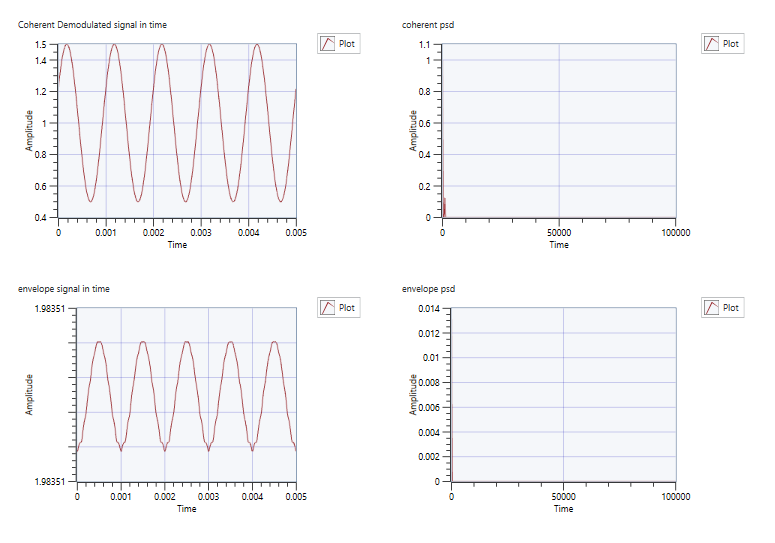
\includegraphics[width=\linewidth]{figures/ex2_amplitude_1.png}
\caption{$A_m=1$ ($\mu=0.5$)}
\label{fig:ex2_am1}
\end{subfigure}
\hfill
\begin{subfigure}{0.49\linewidth}
\centering
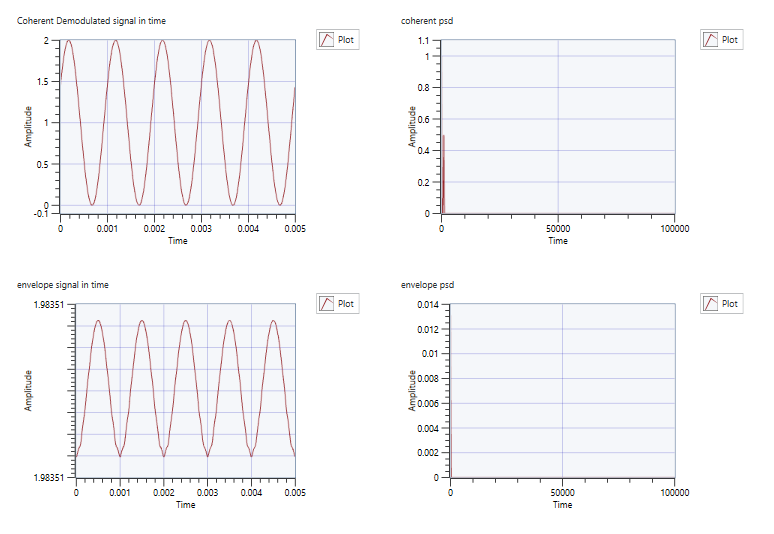
\includegraphics[width=\linewidth]{figures/ex2_amplitude_2.png}
\caption{$A_m=2$ ($\mu=1.0$)}
\label{fig:ex2_am2}
\end{subfigure}

\vspace{0.5em}

\begin{subfigure}{0.49\linewidth}
\centering
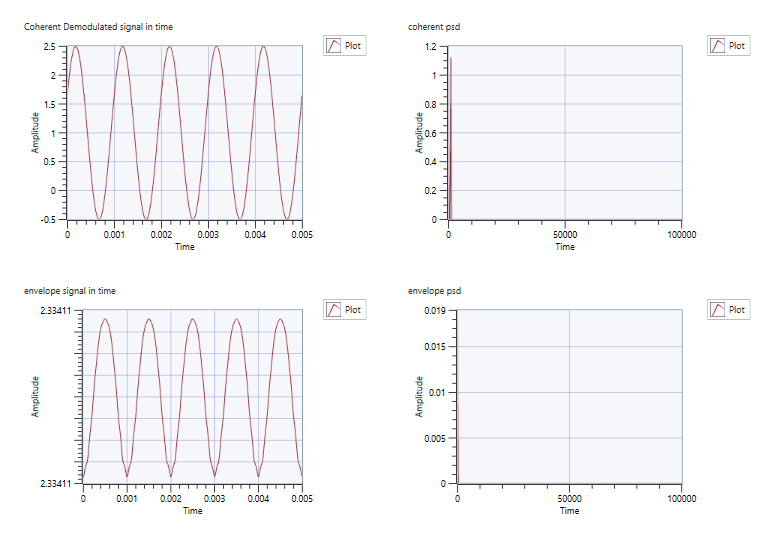
\includegraphics[width=\linewidth]{figures/ex2_amplitude_3.png}
\caption{$A_m=3$ ($\mu=1.5$)}
\label{fig:ex2_am3}
\end{subfigure}
\hfill
\begin{subfigure}{0.49\linewidth}
\centering
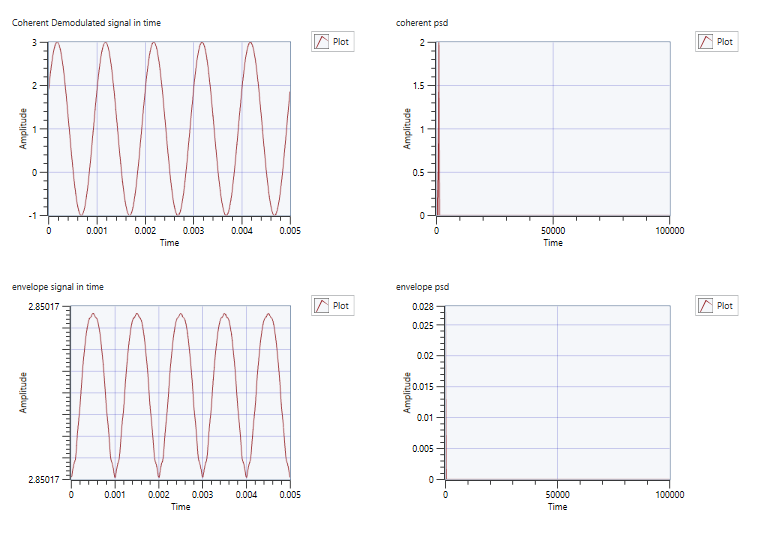
\includegraphics[width=\linewidth]{figures/ex2_amplitude_4.png}
\caption{$A_m=4$ ($\mu=2.0$)}
\label{fig:ex2_am4}
\end{subfigure}
\caption{Demodulated outputs for increasing message amplitude. Each image shows coherent and envelope time/PSD plots.}
\label{fig:ex2_all_cases}
\end{figure}

\subsection*{What Changes Between the Two Demodulation Techniques? Why?}
As $A_m$ increases by 1, the coherent demodulated sinusoid amplitude increases by approximately 0.5. This matches coherent detection scaling:
\begin{equation}
y_{\mathrm{LPF}}(t)\approx \frac{1}{2}\left[A_c + A_m\cos(2\pi f_m t)\right]
\end{equation}
for synchronized carrier recovery. Therefore, the recovered AC term is proportional to $A_m/2$.

The key difference in waveform shape is:
\begin{itemize}
\item \textbf{Coherent demodulation} preserves the signed baseband waveform (positive and negative excursions) after DC removal.
\item \textbf{Envelope detection} mainly preserves amplitude variation (magnitude of the envelope), so the recovered waveform is unipolar/positive-biased.
\end{itemize}

As message amplitude increases, both outputs show larger variation, but envelope detection is constrained by the no-inversion condition $\mu\le 1$. For $\mu>1$ (cases $A_m=3,4$ with $A_c=2$), over-modulation can introduce distortion because rectification cannot recover sign information once the envelope inverts.
